\documentclass[12pt, a4paper]{article}
\usepackage[margin=0.5in]{geometry}
\usepackage[utf8]{inputenc}
\usepackage{amsmath}
\usepackage{amsfonts}
\usepackage{amssymb}
\usepackage{amsthm}

\geometry{
 a4paper,
 left=.5in,
 top=.5in,}


\usepackage{float}
\usepackage{subfigure}
\usepackage{framed}
\usepackage{xcolor}

\usepackage{hyperref}
\hypersetup{
  colorlinks   = true, %Colours links instead of ugly boxes
  urlcolor     = red, %Colour for external hyperlinks
  linkcolor    = black, %Colour of internal links
  citecolor   = blue %Colour of citations
}

\usepackage{graphicx}
\graphicspath{{images/}}

\definecolor{shadecolor}{gray}{0.9}

% Operators
\DeclareMathOperator*{\argmax}{arg\,max}
\DeclareMathOperator*{\argmin}{arg\,min}
\DeclareMathOperator*{\argminA}{arg\,min} % Jan Hlavacek

% Environments theorems
\newtheorem{questions}{Question}
\newenvironment{question}
   {\begin{shaded}\begin{questions}}
   {\end{questions}\end{shaded}}

\renewcommand{\refname}{\normalfont\selectfont\normalsize References} 


\font\myfont=cmr12 at 20pt
\title{\vspace{-1.8cm} \myfont Learning sequence disambiguation with synaptic traces in associative neural networks}
\font\myfont=cmr12 at 12pt
\author{\myfont  Ram\'on Mart\'inez, Anders Lansner, Pawel Herman}


% Paragraph parameters
%\setlength{\parskip}{1em}

\begin{document}
\date{}
\maketitle



\textbf{Summary}. In this work we study the problem of sequence disambiguation in an associative neural network with meta-stable attractor states. The network is capable of encoding sequences with the associative Bayesian Confidence Propagation Neural Network (BCPNN) learning rule through the use of synaptic z-traces. The problem of sequence disambiguation is parameterized by the the overlap in activation between two competing sequences. The sensitivity of the system to noise under various regimes is systematically tested. The network robustly differentiates between considerably overlapping sequences. The performance is non-monotonically modulated by the time constant of synaptic traces and a range for optimal disambiguation is shown as a function of noise level. 

\textbf{Central question.} The disambiguation of sequences with overlaping states of activity using contextual information is a long standing problem in systems neuroscience \cite{levy1996sequence} (see Fig. \ref{fig:results}A-B for examples of sequence disambiguation). Although different neural mechanisms have been proposed in computational modeling, they suffer from either poor disambiguation capabilities, high computational overhead or excessive suceptibility to noise. Following previous work \cite{tully2016spike, lansner2009associative} we propose here an extension of the attractor memory model that learns the sequential structure of the input through the associative BCPNN learning rule and examine its disambiguation capabilities.

 %Some, for example, require the existence of an extra layers or units of contextual code for the dynamical history of the system  \cite{levy1996sequence}, others require persistent activity to last as long as the the disambiguation window   \cite{verduzco2012model},  finally other attempts require the existence of grand-mother-cells with fine-tuned connectivity for each of the specific sequences \cite{wang1990complex}%

%Attractors neural networks provide a computational theory of memory that has proven itself both fruitful and powerful \cite{lansner2009associative}. Early attemps  \cite{amit1992modeling} of using . 

%Our rate based attractor \cite{tully2016spike} \cite{lansner2009associative} network model builds in the spike model to encode the sequential structure model of the input through the associative BCPNN learning rule that exploits synaptic traces. 
\textbf{Approach}. The topological structure of the network is presented in Fig. \ref{fig:model}A. Recurrent connectivity tends to fix patterns of activation in place whereas feed-forward connectivity coupled with adaptation dynamics together with competition initiate pattern transition (meta-stable attractor states). The dynamics of the network are described in detail by the rate-model in Eq. \ref{eq:dynamics} which contains an adaptation term and binary activation units whose sequential dynamics we illustrate in top of Fig. \ref{fig:results}B. The short term dynamical history of the system is preserved in the z-filters (shown in Fig. \ref{fig:model}B, middle) which are low-passed versions of the activation characterized by a time constant $\tau_z$. The z-filters are responsible for both unit activation through the current and learning. Learning works by accumulating evidence of independent and correlated activity of unit activation ($\vec{p}$ and $\mathbf{P}$ respectively) and weighting them against each other to calculate the connectivity matrix as show in Eq. \ref{eq:learning}. The sequential binding of attractors is accomplished by the z-traces (Fig.\ref{fig:model}C) leading to excitatory connectivity  between  contiguously active units. 


\begin{figure}[H]
\centering
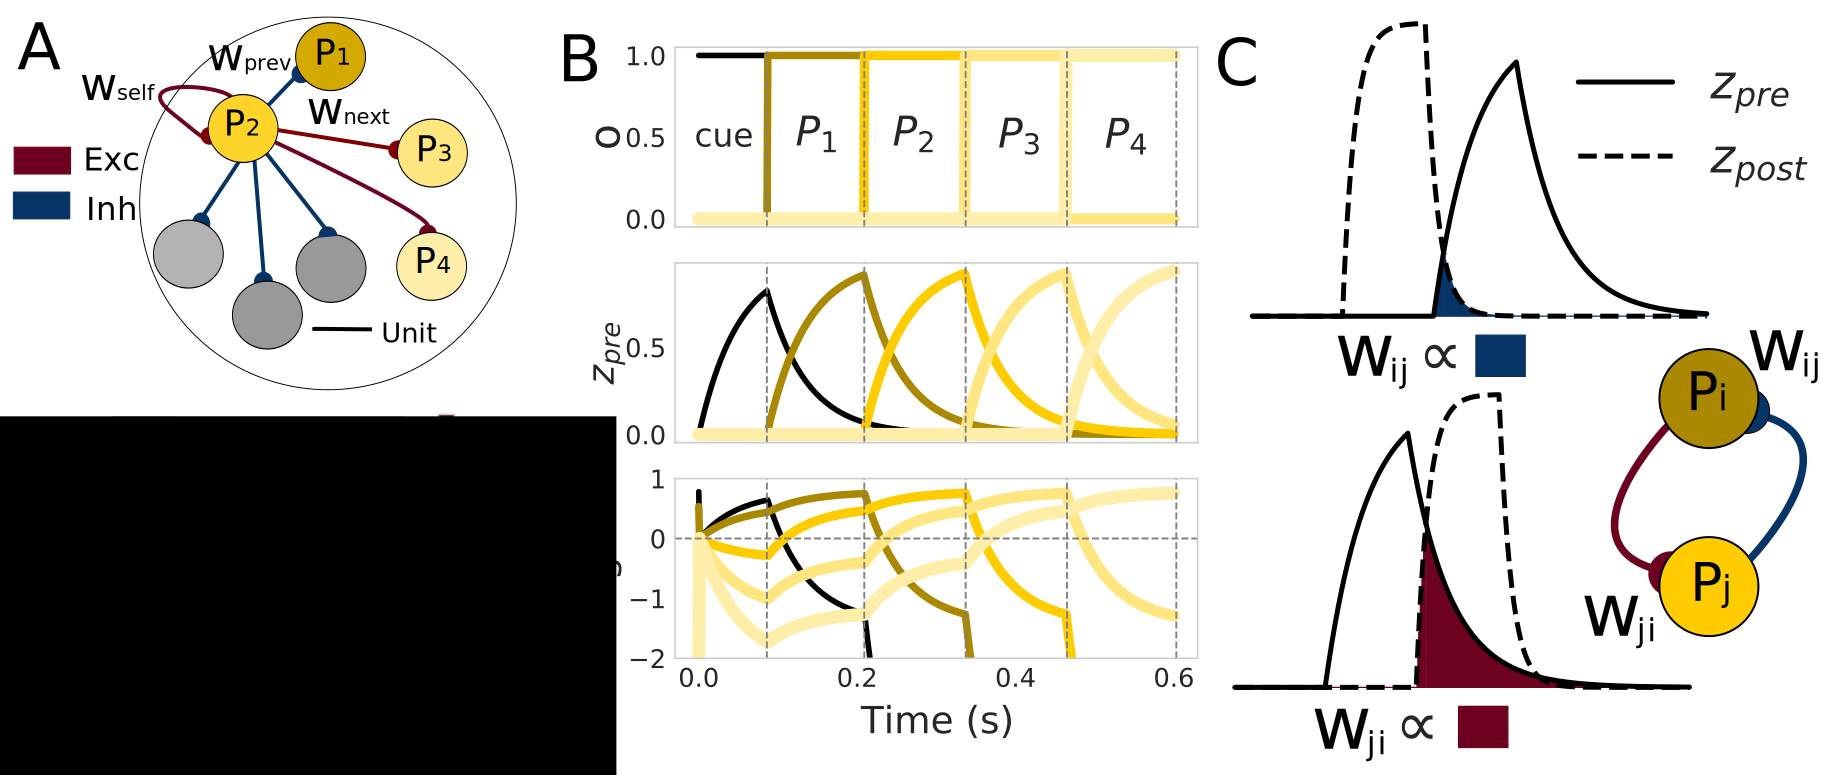
\includegraphics[scale=0.29]{model.png}
\caption{Network: (A) topology (only connections emanating from $P_2$) and weight matrix, (B) dynamics, (C) learning scheme. Overlap of z-traces (red and blue) leads to temporal binding of units.}
\label{fig:model}
\end{figure}

%\begin{figure}[H]
%\centering
%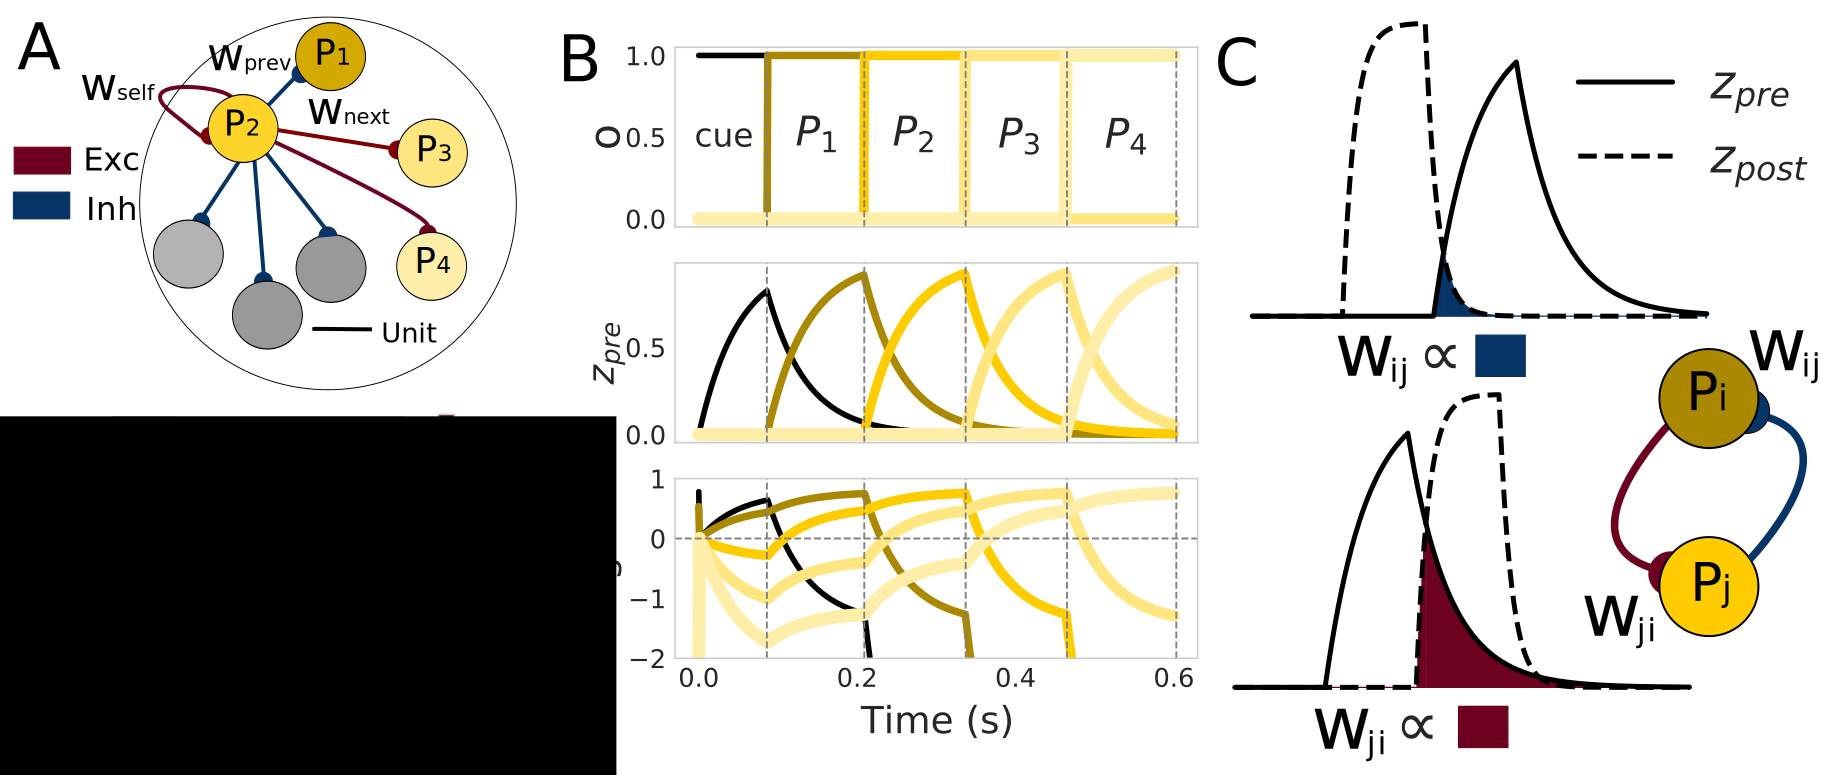
\includegraphics[width=500.0pt, height=190.0pt]{model.png}
%\caption{Network: (A) topology and connectivity (B) network dynamics. (C) learning scheme. Overlap of the z-unit activation (in the right direction) leads to temporal binding of units.}
%\label{fig:model}
%\end{figure}

\begin{align}
\tau_s \dfrac{d \vec{s}}{dt} &=  \mathbf{W} \cdot \vec{\mathbf{z}}_{pre}  - g_a \vec{\mathbf{a}} - \vec{\mathbf{s}}  + \sigma d\vec{\mathbf{\xi}}(t)  
  &\tau_a \dfrac{d\vec{\mathbf{a}}}{dt} &= \vec{\mathbf{o}} - \vec{\mathbf{a}} 
   &o_i &=   \begin{cases}
       1,&  s_i = \underset{hypercolumn}{\max}(\vec{\mathbf{s}}),\\
       0 ,& \text{otherwise}
    \end{cases} \label{eq:dynamics}
\end{align}
\begin{align}
\tau_{z_{pre}} \dfrac{d\vec{\mathbf{\mathbf{z}}}_{pre}}{dt} &= \vec{\mathbf{o}} - \vec{\mathbf{z}}_{pre} 
 & \tau_{z_{post}} \dfrac{d \vec{\mathbf{z}}_{post}}{dt} &= \vec{\mathbf{o}} - \vec{\mathbf{z}}_{post} 
& t \dfrac{d \vec{\mathbf{p}}_{pre}}{dt} &= \vec{\mathbf{z}}_{pre} - \vec{\mathbf{p}}_{pre}  
 \nonumber \\
 t\dfrac{d\mathbf{P}}{dt} &= \vec{\mathbf{p}}_{pre} \otimes \vec{\mathbf{p}}_{post} -\mathbf{P}  
 &t\dfrac{d\vec{\mathbf{p}}_{post}}{dt} &= \vec{\mathbf{z}}_{post} - \vec{\mathbf{p}}_{post}   
 &\mathbf{W} &= \log \left(\frac{\mathbf{P}}{\vec{\mathbf{p}}_{pre} \otimes \vec{\mathbf{p}}_{post}} \right)   \label{eq:learning}
\end{align}

\textbf{Results}
As can be expected, the success rate (successful trials over total trials) depends on the length of the disambiguation window (the number of overlapping sequence components) across different synaptic time constants, $\tau_{z_{pre}}$ (Fig. \ref{fig:results}E). Interestingly, the network’s capability to disambiguate sequences with increasing overlap at least with $0.8$ success rate does not monotonically grow with $\tau_{z_{pre}}$(Fig. \ref{fig:results}) but shows an U-shape with a limited value of optimal conditions for sequence disambiguation. This stems from the interaction of two competing mechanisms: 1) for low values of $\tau_{z_{pre}}$ the z-traces are not active long enough to bridge the required sequence overlap whereas longer values of $\tau_{z_{pre}}$ lead to non-differentiating learning among the sequence (homogeneous weights structure). 


\begin{figure}[H]
\centering
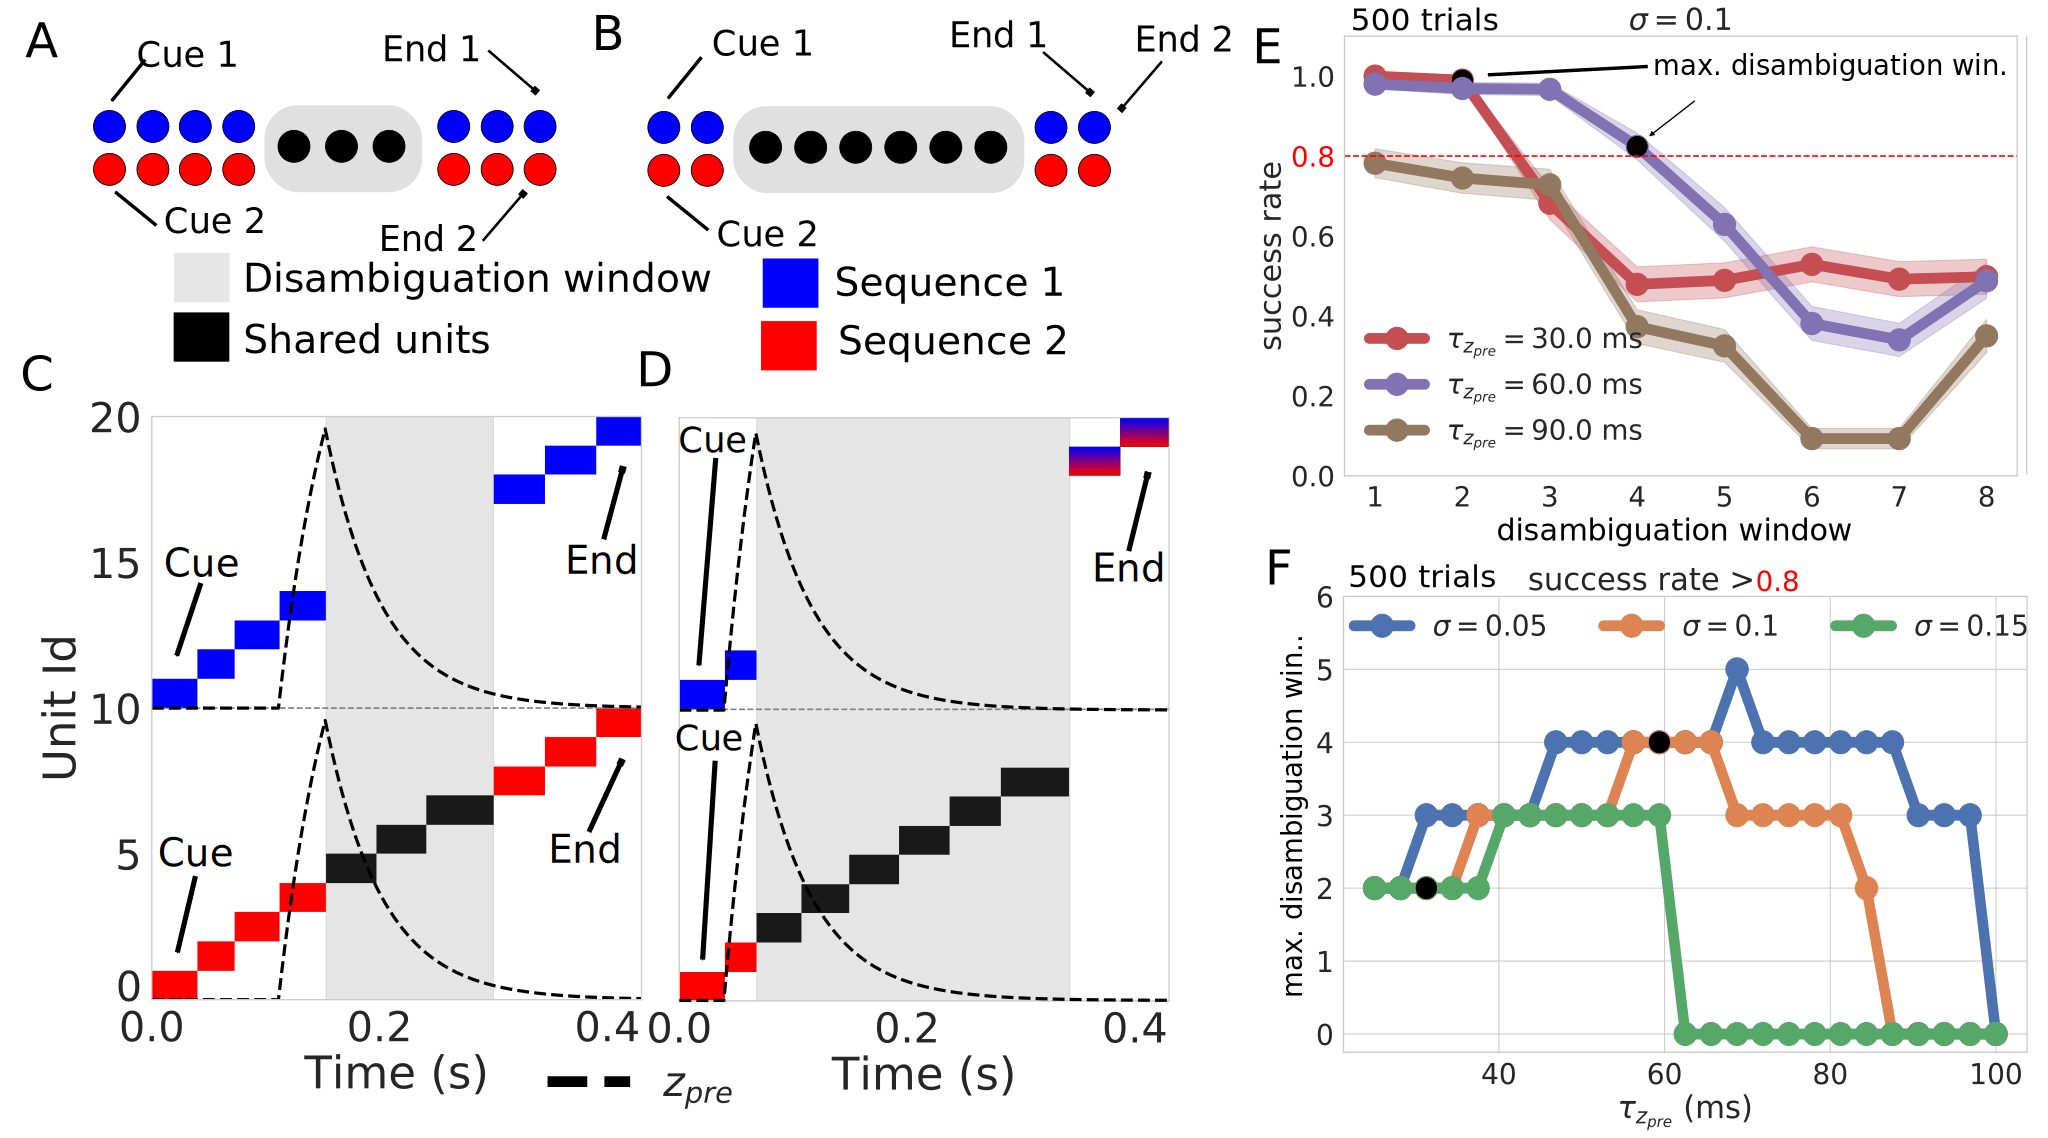
\includegraphics[scale=0.25]{results.png}
\caption{Schematic of the sequence disambiguation problem with either short (A) or long (B) overlap. Short overlap is successfully bridged by the synaptic trace resulting from the unit activation prior to the overlapping component resulting in successful recall of the correct sequence (C). The longer overlap cannot be bridged, which results in unsuccessful sequence disambiguation (D). (E) Success rate of disambiguation (over 500 trials) for varying size of sequence overlap and $\tau_{z_{pre}}$under noise corresponding to $\sigma = 0.1$.  (F) The effect of $\tau_{z_{pre}}$ on the max sequence overlap in a disambiguation task allowing for at least 0.8 success rate under varying noise conditions.}
\label{fig:results}
\end{figure}

\textbf{Conclusions}. The proposed synaptic trace based BCPNN learning in an attractor network model allows for encoding and successful recall of largely overlapping sequences even in noisy conditions. The upper limit of the overlap window length for successful disambiguation is non-linearly dependent on the time constant of the synaptic traces and monotonically decreases with rising noise levels

%\begin{align}
%\tau_s \dfrac{ds_i}{dt} &=  \sum_{j} w_{ij} z_j  - g_a a_i - s_i  + \sigma d\xi(t)  
%  &\tau_a \dfrac{da_i}{dt} &= o_i - a_i  &o_i =   \begin{cases}
%       1,&  s_i = \underset{hypercolumn}{\max}(\mathbf{s}),\\
%       0 ,& \text{otherwise}
%    \end{cases} \label{eq:dynamics}
%\end{align}
%
%\begin{align}
%\tau_{z_{pre}} \dfrac{dz_i}{dt} &= o_i - z_i 
%& \tau_{z_{post}} \dfrac{d z_j}{dt} &= o_j - z_j 
%&t \dfrac{dp_i}{dt} &= z_i - p_i  
%&t\dfrac{dp_{ij}}{dt} = z_i z_j - p_{ij} \nonumber \\
%&t\dfrac{dp_j}{dt} = z_j - p_j   
%&w_{ij} &= \log \left(\frac{p_{ij}}{p_i p_j} \right) & \beta_i &= \log(p_i)  \label{eq:learning}
%\end{align}

\bibliographystyle{plain}
\bibliography{short.bib}

\end{document}